\documentclass[12pt]{article}
\usepackage[letterpaper]{geometry}
\usepackage{fullpage}
\usepackage[hidelinks]{hyperref}
\usepackage{fancyvrb}
\usepackage{color}
\usepackage{textcomp}
\usepackage{upquote}
\usepackage[none]{hyphenat}
\usepackage{graphicx}

\title{EECS 581 Senior Design Capstone Project Proposal \\
busbus: All transit data, one interface}
\author{Nick Gilliland, Alex Gustafson, Zane Ralston, Monica Shafii, Ian Weller \\ \url{spaceboats.github.io}}

\setlength{\parindent}{0.0in}
\setlength{\parskip}{0.125in}


\begin{document}
\maketitle

\section{Abstract}

The spaceboats senior design group is developing a common platform for accessing mass-transit data
across multiple agencies with different APIs and data formats.
We intend to demonstrate the desired functionality (a convenient open-source data tool
for developers) by building projects on top of the platform, such as a web application, an Android app, and
an LED board that shows data about upcoming buses.

\section{Specific Aims}

The busbus platform aims to provide a Python API and web API for developers to access
mass-transit data, both static and realtime (where available), from all existing agencies worldwide
under a common interface.
The platform will be open source and freely licensed, so developers can create new and exciting projects
with simple access to open transit data, as well as extend support in busbus for new transit agencies.
The goal is for
developers to be able to focus on their applications instead of putting a considerable amount of
effort into how to access specific information from each agency's API, or how to transform
the returned data into a consistent format.

\section{Existing Transit Data Work}
There are a lot of existing standards and services built around transit data.
However, none of them simplify the process for developers of dealing with multiple transit agencies.

It's important to note that the busbus platform is \textit{not} attempting to be a new transit data standard ---
we want to leverage existing APIs and make them more easily accessible for programmers.

\subsection{Current Standards}
The General Transit Feed Specification (GTFS)\footnote{Google, \textit{General Transit Feed Specification},
\url{https://developers.google.com/transit/gtfs/}},
developed by Google and TriMet in 2005, has become the industry standard for static transit data.
The data is designed to be readable by anything --- simple CSV files in a Zip archive ---
but in practice, \textit{using} the data is more difficult compared to a relational database
or an object-oriented API.

In addition, GTFS doesn't have realtime data. GTFS-realtime is a specification built to add
realtime data, but it's not widely used. Larger North American transit agencies provide
data in this format but also their own, richer realtime data APIs.

\subsection{Agency-Specific APIs}

Numerous agency-specific APIs exist for mass-transit in metropolitan areas.
These may be sufficient if developers are only looking to create an application with a local scope. However,
a common goal of developers is to write code as a foundation to be built upon that is not unnecessarily limited,
but is useful to our peers, and prevents the cost of effort put into the same
problem again and again.

In referencing even a few of the existing agency-specific APIs, it
becomes apparent that the data that can be accessed, and the format of the data returned, 
vary greatly. The CTA Bus Tracker API provides vehicle locations, route data, prediction data and 
service bulletins and returns this data in XML and other formats.\footnote{Chicago Transit Authority (CTA), \textit{Bus Tracker API Documentation},
\url{http://www.transitchicago.com/assets/1/developer\_center/BusTime\_Developer\_API\_Guide.pdf}} The MBTA Real-Time API provides
stops by location, routes by stop, predictions by stop, alert headers, and alerts by ID, and returns
this data in XML and JSON formats.\footnote{Massachusetts Bay Transit Authority (MBTA), \textit{MBTA-Realltime Quick-Start Guide},
\url{http://realtime.mbta.com/Portal/Content/Documents/MBTA-realtime\_APIQuickStart\_2014-08-04.pdf}}

\subsection{Multi-Agency APIs and Apps}
There exist APIs and services that attempt to unify access to data over agency-specific APIs.
However, these generally either encompass a limited number of agencies or a limited set of
data from each agency, and are often not open APIs at all.

The NextBus API only provides data for
around 50 agencies within the U.S. and Canada, and for the most part, only provides bus data 
and not data for other forms of transportation.\footnote{NextBus, \textit{API Portal},
	\url{http://api-portal.anypoint.mulesoft.com/nextbus/api/nextbus-api}}

The Transit App covers data for 200+ agencies
and 86 global metropolitan areas, but is a mobile application and doesn't provide an open API for developers to retrieve the
data.\footnote{Transit App, \textit{Regions}, \url{http://thetransitapp.com/regions}}


\section{Proposed Solution and Preliminary Design}
\subsection{Python Library}
The bulk of our proposed project is a Python library which allows the user to get various transit data.
We currently intend to provide support for \textit{agencies}, \textit{routes}, \textit{stops}, and \textit{arrivals}.
Each of these entities will provide all the data busbus knows about; for instance, an Arrival can have both a scheduled arrival time
and a prediction based on the current location of a vehicle.

The API is still in flux, but we're intending to have interactions with it looking something like figure~\ref{fig:pythonsample}.

\begin{figure}[h]
	\begin{center}
		\makeatletter
\def\PY@reset{\let\PY@it=\relax \let\PY@bf=\relax%
    \let\PY@ul=\relax \let\PY@tc=\relax%
    \let\PY@bc=\relax \let\PY@ff=\relax}
\def\PY@tok#1{\csname PY@tok@#1\endcsname}
\def\PY@toks#1+{\ifx\relax#1\empty\else%
    \PY@tok{#1}\expandafter\PY@toks\fi}
\def\PY@do#1{\PY@bc{\PY@tc{\PY@ul{%
    \PY@it{\PY@bf{\PY@ff{#1}}}}}}}
\def\PY#1#2{\PY@reset\PY@toks#1+\relax+\PY@do{#2}}

\expandafter\def\csname PY@tok@gd\endcsname{\def\PY@tc##1{\textcolor[rgb]{0.63,0.00,0.00}{##1}}}
\expandafter\def\csname PY@tok@gu\endcsname{\let\PY@bf=\textbf\def\PY@tc##1{\textcolor[rgb]{0.50,0.00,0.50}{##1}}}
\expandafter\def\csname PY@tok@gt\endcsname{\def\PY@tc##1{\textcolor[rgb]{0.00,0.27,0.87}{##1}}}
\expandafter\def\csname PY@tok@gs\endcsname{\let\PY@bf=\textbf}
\expandafter\def\csname PY@tok@gr\endcsname{\def\PY@tc##1{\textcolor[rgb]{1.00,0.00,0.00}{##1}}}
\expandafter\def\csname PY@tok@cm\endcsname{\let\PY@it=\textit\def\PY@tc##1{\textcolor[rgb]{0.25,0.50,0.50}{##1}}}
\expandafter\def\csname PY@tok@vg\endcsname{\def\PY@tc##1{\textcolor[rgb]{0.10,0.09,0.49}{##1}}}
\expandafter\def\csname PY@tok@m\endcsname{\def\PY@tc##1{\textcolor[rgb]{0.40,0.40,0.40}{##1}}}
\expandafter\def\csname PY@tok@mh\endcsname{\def\PY@tc##1{\textcolor[rgb]{0.40,0.40,0.40}{##1}}}
\expandafter\def\csname PY@tok@go\endcsname{\def\PY@tc##1{\textcolor[rgb]{0.53,0.53,0.53}{##1}}}
\expandafter\def\csname PY@tok@ge\endcsname{\let\PY@it=\textit}
\expandafter\def\csname PY@tok@vc\endcsname{\def\PY@tc##1{\textcolor[rgb]{0.10,0.09,0.49}{##1}}}
\expandafter\def\csname PY@tok@il\endcsname{\def\PY@tc##1{\textcolor[rgb]{0.40,0.40,0.40}{##1}}}
\expandafter\def\csname PY@tok@cs\endcsname{\let\PY@it=\textit\def\PY@tc##1{\textcolor[rgb]{0.25,0.50,0.50}{##1}}}
\expandafter\def\csname PY@tok@cp\endcsname{\def\PY@tc##1{\textcolor[rgb]{0.74,0.48,0.00}{##1}}}
\expandafter\def\csname PY@tok@gi\endcsname{\def\PY@tc##1{\textcolor[rgb]{0.00,0.63,0.00}{##1}}}
\expandafter\def\csname PY@tok@gh\endcsname{\let\PY@bf=\textbf\def\PY@tc##1{\textcolor[rgb]{0.00,0.00,0.50}{##1}}}
\expandafter\def\csname PY@tok@ni\endcsname{\let\PY@bf=\textbf\def\PY@tc##1{\textcolor[rgb]{0.60,0.60,0.60}{##1}}}
\expandafter\def\csname PY@tok@nl\endcsname{\def\PY@tc##1{\textcolor[rgb]{0.63,0.63,0.00}{##1}}}
\expandafter\def\csname PY@tok@nn\endcsname{\let\PY@bf=\textbf\def\PY@tc##1{\textcolor[rgb]{0.00,0.00,1.00}{##1}}}
\expandafter\def\csname PY@tok@no\endcsname{\def\PY@tc##1{\textcolor[rgb]{0.53,0.00,0.00}{##1}}}
\expandafter\def\csname PY@tok@na\endcsname{\def\PY@tc##1{\textcolor[rgb]{0.49,0.56,0.16}{##1}}}
\expandafter\def\csname PY@tok@nb\endcsname{\def\PY@tc##1{\textcolor[rgb]{0.00,0.50,0.00}{##1}}}
\expandafter\def\csname PY@tok@nc\endcsname{\let\PY@bf=\textbf\def\PY@tc##1{\textcolor[rgb]{0.00,0.00,1.00}{##1}}}
\expandafter\def\csname PY@tok@nd\endcsname{\def\PY@tc##1{\textcolor[rgb]{0.67,0.13,1.00}{##1}}}
\expandafter\def\csname PY@tok@ne\endcsname{\let\PY@bf=\textbf\def\PY@tc##1{\textcolor[rgb]{0.82,0.25,0.23}{##1}}}
\expandafter\def\csname PY@tok@nf\endcsname{\def\PY@tc##1{\textcolor[rgb]{0.00,0.00,1.00}{##1}}}
\expandafter\def\csname PY@tok@si\endcsname{\let\PY@bf=\textbf\def\PY@tc##1{\textcolor[rgb]{0.73,0.40,0.53}{##1}}}
\expandafter\def\csname PY@tok@s2\endcsname{\def\PY@tc##1{\textcolor[rgb]{0.73,0.13,0.13}{##1}}}
\expandafter\def\csname PY@tok@vi\endcsname{\def\PY@tc##1{\textcolor[rgb]{0.10,0.09,0.49}{##1}}}
\expandafter\def\csname PY@tok@nt\endcsname{\let\PY@bf=\textbf\def\PY@tc##1{\textcolor[rgb]{0.00,0.50,0.00}{##1}}}
\expandafter\def\csname PY@tok@nv\endcsname{\def\PY@tc##1{\textcolor[rgb]{0.10,0.09,0.49}{##1}}}
\expandafter\def\csname PY@tok@s1\endcsname{\def\PY@tc##1{\textcolor[rgb]{0.73,0.13,0.13}{##1}}}
\expandafter\def\csname PY@tok@sh\endcsname{\def\PY@tc##1{\textcolor[rgb]{0.73,0.13,0.13}{##1}}}
\expandafter\def\csname PY@tok@sc\endcsname{\def\PY@tc##1{\textcolor[rgb]{0.73,0.13,0.13}{##1}}}
\expandafter\def\csname PY@tok@sx\endcsname{\def\PY@tc##1{\textcolor[rgb]{0.00,0.50,0.00}{##1}}}
\expandafter\def\csname PY@tok@bp\endcsname{\def\PY@tc##1{\textcolor[rgb]{0.00,0.50,0.00}{##1}}}
\expandafter\def\csname PY@tok@c1\endcsname{\let\PY@it=\textit\def\PY@tc##1{\textcolor[rgb]{0.25,0.50,0.50}{##1}}}
\expandafter\def\csname PY@tok@kc\endcsname{\let\PY@bf=\textbf\def\PY@tc##1{\textcolor[rgb]{0.00,0.50,0.00}{##1}}}
\expandafter\def\csname PY@tok@c\endcsname{\let\PY@it=\textit\def\PY@tc##1{\textcolor[rgb]{0.25,0.50,0.50}{##1}}}
\expandafter\def\csname PY@tok@mf\endcsname{\def\PY@tc##1{\textcolor[rgb]{0.40,0.40,0.40}{##1}}}
\expandafter\def\csname PY@tok@err\endcsname{\def\PY@bc##1{\setlength{\fboxsep}{0pt}\fcolorbox[rgb]{1.00,0.00,0.00}{1,1,1}{\strut ##1}}}
\expandafter\def\csname PY@tok@kd\endcsname{\let\PY@bf=\textbf\def\PY@tc##1{\textcolor[rgb]{0.00,0.50,0.00}{##1}}}
\expandafter\def\csname PY@tok@ss\endcsname{\def\PY@tc##1{\textcolor[rgb]{0.10,0.09,0.49}{##1}}}
\expandafter\def\csname PY@tok@sr\endcsname{\def\PY@tc##1{\textcolor[rgb]{0.73,0.40,0.53}{##1}}}
\expandafter\def\csname PY@tok@mo\endcsname{\def\PY@tc##1{\textcolor[rgb]{0.40,0.40,0.40}{##1}}}
\expandafter\def\csname PY@tok@kn\endcsname{\let\PY@bf=\textbf\def\PY@tc##1{\textcolor[rgb]{0.00,0.50,0.00}{##1}}}
\expandafter\def\csname PY@tok@mi\endcsname{\def\PY@tc##1{\textcolor[rgb]{0.40,0.40,0.40}{##1}}}
\expandafter\def\csname PY@tok@gp\endcsname{\let\PY@bf=\textbf\def\PY@tc##1{\textcolor[rgb]{0.00,0.00,0.50}{##1}}}
\expandafter\def\csname PY@tok@o\endcsname{\def\PY@tc##1{\textcolor[rgb]{0.40,0.40,0.40}{##1}}}
\expandafter\def\csname PY@tok@kr\endcsname{\let\PY@bf=\textbf\def\PY@tc##1{\textcolor[rgb]{0.00,0.50,0.00}{##1}}}
\expandafter\def\csname PY@tok@s\endcsname{\def\PY@tc##1{\textcolor[rgb]{0.73,0.13,0.13}{##1}}}
\expandafter\def\csname PY@tok@kp\endcsname{\def\PY@tc##1{\textcolor[rgb]{0.00,0.50,0.00}{##1}}}
\expandafter\def\csname PY@tok@w\endcsname{\def\PY@tc##1{\textcolor[rgb]{0.73,0.73,0.73}{##1}}}
\expandafter\def\csname PY@tok@kt\endcsname{\def\PY@tc##1{\textcolor[rgb]{0.69,0.00,0.25}{##1}}}
\expandafter\def\csname PY@tok@ow\endcsname{\let\PY@bf=\textbf\def\PY@tc##1{\textcolor[rgb]{0.67,0.13,1.00}{##1}}}
\expandafter\def\csname PY@tok@sb\endcsname{\def\PY@tc##1{\textcolor[rgb]{0.73,0.13,0.13}{##1}}}
\expandafter\def\csname PY@tok@k\endcsname{\let\PY@bf=\textbf\def\PY@tc##1{\textcolor[rgb]{0.00,0.50,0.00}{##1}}}
\expandafter\def\csname PY@tok@se\endcsname{\let\PY@bf=\textbf\def\PY@tc##1{\textcolor[rgb]{0.73,0.40,0.13}{##1}}}
\expandafter\def\csname PY@tok@sd\endcsname{\let\PY@it=\textit\def\PY@tc##1{\textcolor[rgb]{0.73,0.13,0.13}{##1}}}

\def\PYZbs{\char`\\}
\def\PYZus{\char`\_}
\def\PYZob{\char`\{}
\def\PYZcb{\char`\}}
\def\PYZca{\char`\^}
\def\PYZam{\char`\&}
\def\PYZlt{\char`\<}
\def\PYZgt{\char`\>}
\def\PYZsh{\char`\#}
\def\PYZpc{\char`\%}
\def\PYZdl{\char`\$}
\def\PYZhy{\char`\-}
\def\PYZsq{\textquotesingle}
\def\PYZdq{\char`\"}
\def\PYZti{\char`\~}
% for compatibility with earlier versions
\def\PYZat{@}
\def\PYZlb{[}
\def\PYZrb{]}
\makeatother
\begin{Verbatim}[commandchars=\\\{\}]
\PY{k+kn}{import} \PY{n+nn}{itertools}
\PY{k+kn}{from} \PY{n+nn}{busbus.provider.mvtransit} \PY{k+kn}{import} \PY{n}{LawrenceTransitProvider}
\PY{n}{lfk} \PY{o}{=} \PY{n}{LawrenceTransitProvider}\PY{p}{(}\PY{p}{)}

\PY{c}{\PYZsh{} Filter for arrivals for the 15th at Spahr stop}
\PY{n}{arr} \PY{o}{=} \PY{n}{lfk}\PY{o}{.}\PY{n}{arrivals}\PY{o}{.}\PY{n}{where}\PY{p}{(}\PY{k}{lambda} \PY{n}{a}\PY{p}{:} \PY{n}{a}\PY{o}{.}\PY{n}{stop}\PY{o}{.}\PY{n}{id} \PY{o}{==} \PY{l+s}{\PYZsq{}}\PY{l+s}{15TH\PYZus{}SPAHR\PYZus{}WB}\PY{l+s}{\PYZsq{}}\PY{p}{)}
\PY{c}{\PYZsh{} Filter for arrivals happening in the next hour}
\PY{n}{arr} \PY{o}{=} \PY{n}{arr}\PY{o}{.}\PY{n}{where}\PY{p}{(}\PY{k}{lambda} \PY{n}{a}\PY{p}{:} \PY{n}{a}\PY{o}{.}\PY{n}{time}\PY{o}{.}\PY{n}{delta} \PY{o}{\PYZlt{}}\PY{o}{=} \PY{l+m+mi}{3600}\PY{p}{)}
\PY{c}{\PYZsh{} Limit to the first 5 arrivals}
\PY{n}{arr} \PY{o}{=} \PY{n}{itertools}\PY{o}{.}\PY{n}{islice}\PY{p}{(}\PY{n}{arr}\PY{p}{,} \PY{l+m+mi}{5}\PY{p}{)}

\PY{k}{for} \PY{n}{arrival} \PY{o+ow}{in} \PY{n}{arr}\PY{p}{:}
    \PY{k}{print}\PY{p}{(}\PY{l+s}{\PYZsq{}}\PY{l+s}{\PYZob{}0\PYZcb{} to \PYZob{}1\PYZcb{} \PYZob{}2\PYZcb{}}\PY{l+s}{\PYZsq{}}\PY{o}{.}\PY{n}{format}\PY{p}{(}\PY{n}{arrival}\PY{o}{.}\PY{n}{route}\PY{o}{.}\PY{n}{name}\PY{p}{,}
                                  \PY{n}{arrival}\PY{o}{.}\PY{n}{route}\PY{o}{.}\PY{n}{direction}\PY{p}{,}
                                  \PY{n}{arrival}\PY{o}{.}\PY{n}{time}\PY{o}{.}\PY{n}{humanize}\PY{p}{(}\PY{p}{)}\PY{p}{)}\PY{p}{)}
\end{Verbatim}

	\end{center}
	\caption{Proposed sample code for interacting with the \texttt{busbus} Python module}
	\label{fig:pythonsample}
\end{figure}

\subsection{Projects}
We intend to build projects on top of the busbus platform.
We want to show our API works as intended, and possibly
fine-tune it in the process --- in a sense, these are some of our test cases. We also want
to demonstrate the actual application of the tool we are building, and how our peers
could possibly use it.

\subsubsection{LED board}
The LED board has already been purchased and assembled. It consists of three smaller LED boards that have been linked together and a Raspberry Pi that controls them.
The three LED boards along with the Raspberry Pi were mounted on a piece of plexiglass.
The Rasberry Pi runs a controller that we wrote\footnote{spaceboats/3001-ledboard on GitHub, \url{https://github.com/spaceboats/3001-ledboard}}
that will parse commands given in JSON.
An example of a command that can be used to
make the board display a solid color is:

\begin{verbatim}
curl -X POST -H "Content-type:application/json" -d \
    '{"mode":"fill", "color":[0, 0, 255]}' \
    http://3001-ledboard.local:8080/state
\end{verbatim}

To integrate this into our project
we will have it display data that we will be getting from busbus.  This will allow
us to show different information about any stop in the world (that
busbus supports). The end goal for the LED board is to show the next few buses that will arrive outside Eaton Hall.

\subsubsection{Web application}
The web application will allow users to view all stops and all bus locations within a small area, city, or world.
There are many ideas that could be implemented in this application. Some of which include:

\begin{itemize}
    \item Drop pins on a map of cities/areas that busbus supports.
    \item Be able to click on stop pins to see which bus numbers and what time the next buses will be there.
    \item Be able to drop pins of bus locations on a map and dynamically update them every few seconds.
    \item Some sort of weird transit game. For example, be able to walk around a map and get on live buses.
\end{itemize}

\subsubsection{Android application}
The Android application will allow users to either select a stop or find bus stops near them using their GPS location.
Once users have found the stop that they want, they will be able to view upcoming scheduled arrival times and
predicted realtime bus arrivals, if realtime data is available for that transit agency. Users will also be able
to save stops, so the stops that they use frequently will be readily available.

Ease of use is important
for showing off the capability of the busbus platform so a high quality user interface will be a priority.
Development of this application will be done using Android Studio.

The Android application will most likely never
be put on the Google Play store because it would require us to host a service, which is outside the scope of this
project; we instead intend to open source it and provide it as a starting base for others.
At this time we plan to only support Android version 4.4 and later to help speed up development time.

\section{Milestones and Schedule}
Our Gantt chart is available online at \url{http://spaceboats.github.io/static/gantt.html}.
An absolutely terrible screenshot is available in section~\ref{app:gantt}, \textit{\nameref{app:gantt}}, as requested --- but you really want to look at the online version.

\section{Tools/Cost Estimate}
\subsection{Tools and language}
The busbus platform will support Python 2.7 and Python 3.3 or later. We're most likely utilizing the following
libraries and modules:
\begin{itemize}
	\item \texttt{requests} (proper HTTP handling)
	\item \texttt{arrow} (proper timezone handling)
	\item \texttt{CherryPy} (for the web server)
	\item \texttt{gevent} (for asynchronous message handling, so data consumers can subscribe to events
		without having to make repeated API calls)
\end{itemize}

\subsection{Hardware}
The only hardware we are using is for the LED board project and has already been purchased, with a final cost of approximately \$230.
\begin{itemize}
\item Raspberry Pi Model B+ 512MB RAM (\$39.95)
\item Raspberry Pi B+ Frosted White Enclosure (\$8.95)
\item SD/MicroSD Memory Card (4 GB SDHC) (\$7.95)
\item 5V 1A (1000mA) USB port power supply - UL Listed (\$5.95)
\item USB cable - A/MicroB (\$3.95)
\item Assembled Pi Cobbler Plus - Breakout Cable for Raspberry Pi B+ (\$6.95)
\item Medium 16x32 RGB LED matrix panel × 3 at \$24.95 each (\$74.85)
\item 5V 10A switching power supply (\$25.00)
\item Female DC Power adapter - 2.1mm jack to screw terminal block (\$2.00)
\item Mounting hardware (approx. \$55.00)
\end{itemize}

\pagebreak

\section{Appendix: Gantt chart}
\label{app:gantt}

The actually-readable version of this chart is available at \url{http://spaceboats.github.io/static/gantt.html}.

Since this could change in the future, this exact version is available at: \\
\url{http://htmlpreview.github.io/?https://github.com/spaceboats/spaceboats.github.io/blob/6b9779ef5f581b9c57b8673445819c3283871bd5/static/gantt.html}

\begin{figure}[h]
	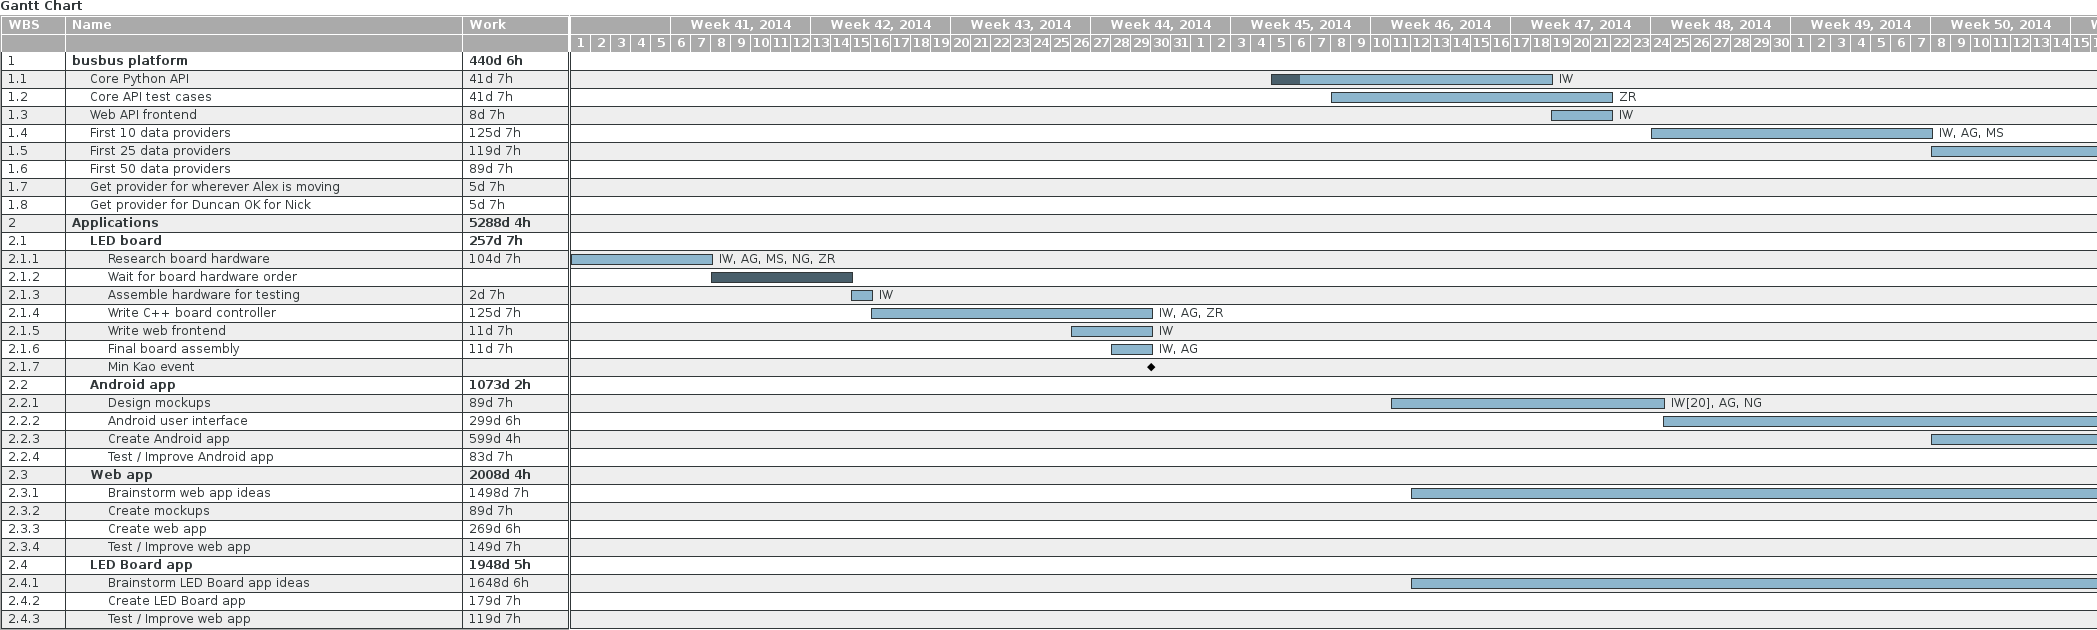
\includegraphics[width=\textwidth]{gantt1.png}
	\\
	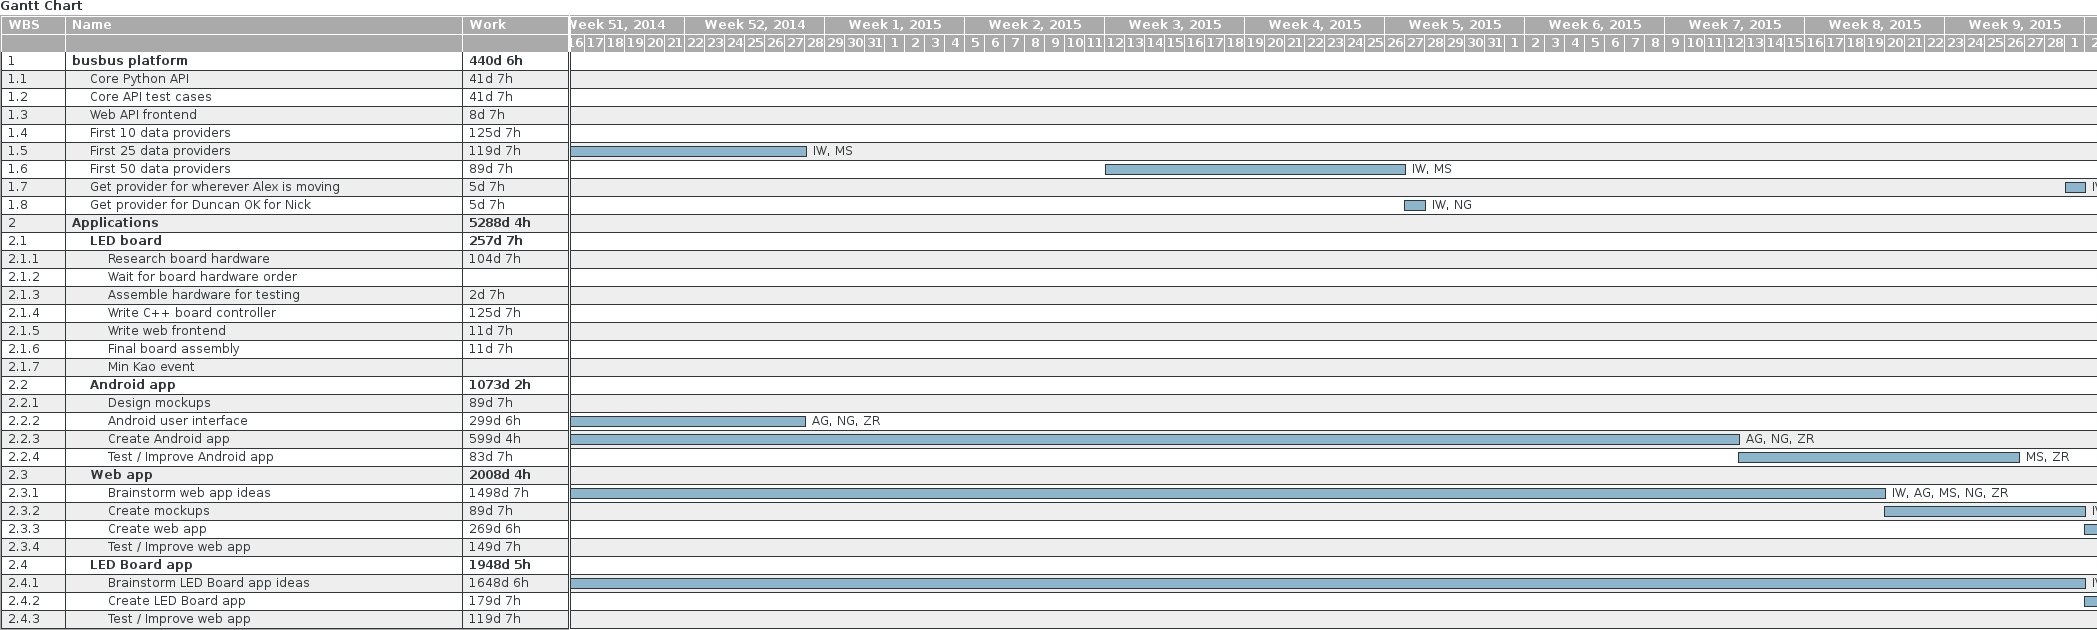
\includegraphics[width=\textwidth]{gantt2.png}
	\\
	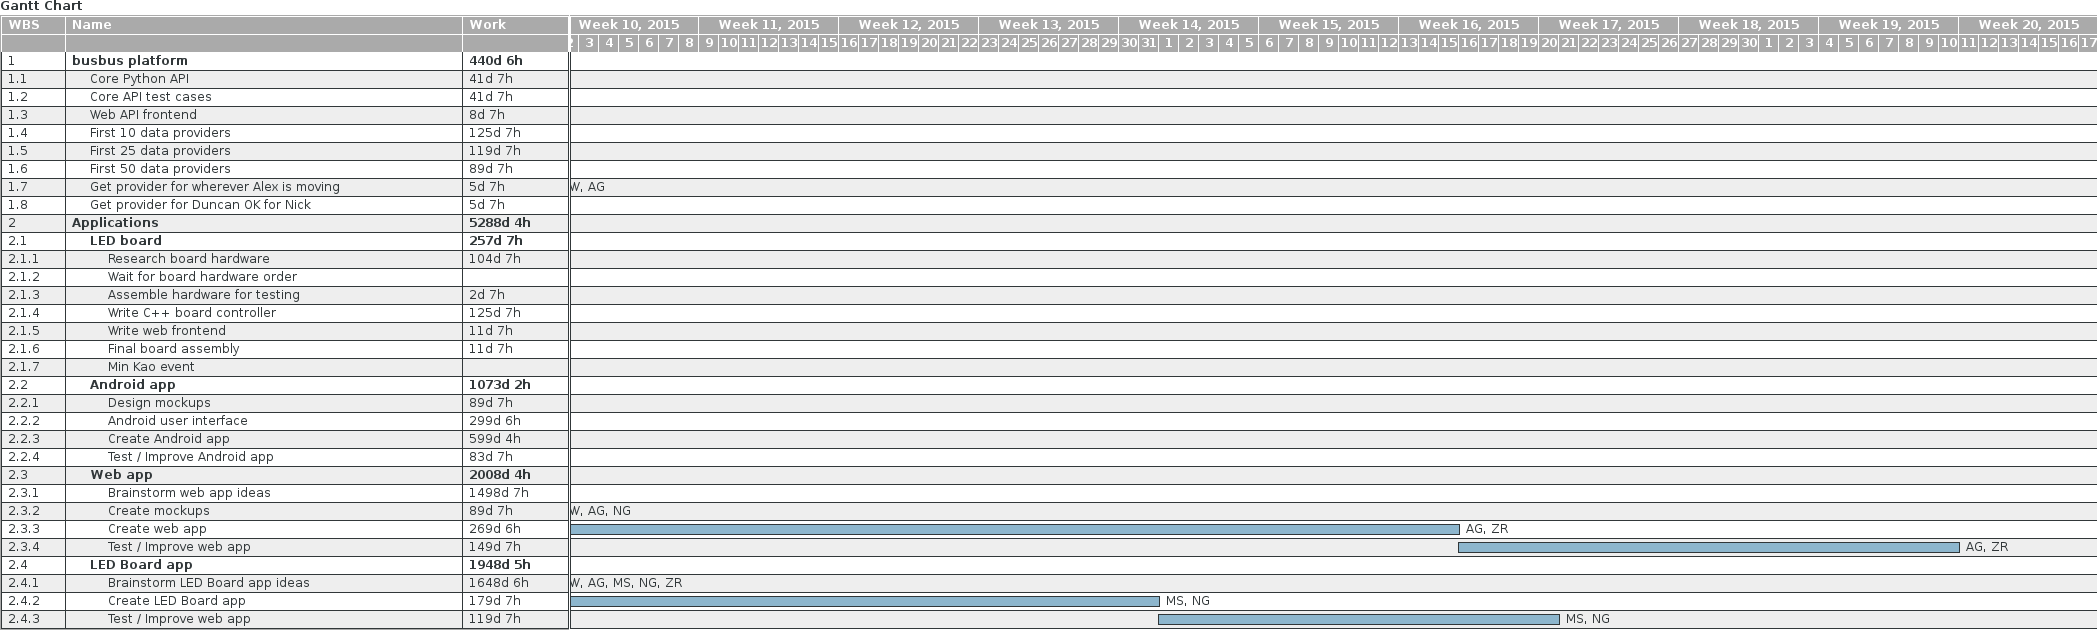
\includegraphics[width=\textwidth]{gantt3.png}
\end{figure}

\end{document}
